\documentclass[11pt,letterpaper]{article}

% --- Packages ---
\usepackage[margin=1in, headheight=24pt]{geometry}
\usepackage{graphicx}
\usepackage{hyperref}
\usepackage{enumitem}
\usepackage{booktabs}
\usepackage{xcolor}
\usepackage{tcolorbox}
\usepackage{fancyhdr}
\usepackage{titlesec}
\usepackage{parskip}
\usepackage[T1]{fontenc}
\usepackage[utf8]{inputenc}
\usepackage{amssymb}
\usepackage{amsmath}
\usepackage{tabularx}
\usepackage{tikz}
\usetikzlibrary{positioning, arrows.meta, calc, decorations.pathreplacing, fit, backgrounds}

% --- Colors ---
\definecolor{minesblue}{RGB}{33,69,126}
\definecolor{minesgold}{RGB}{204,174,0}
\definecolor{tipgreen}{RGB}{34,120,58}
\definecolor{warnred}{RGB}{180,30,30}
\definecolor{lightgray}{RGB}{245,245,245}
\definecolor{vdefine}{RGB}{41,98,163}
\definecolor{vdesign}{RGB}{33,69,126}
\definecolor{vbuild}{RGB}{90,90,90}
\definecolor{vverify}{RGB}{34,120,58}

% --- Hyperref Setup ---
\hypersetup{
    colorlinks=true,
    linkcolor=minesblue,
    urlcolor=minesblue,
    citecolor=minesblue
}

% --- Header/Footer ---
\pagestyle{fancy}
\fancyhf{}
\fancyhead[L]{\textcolor{minesblue}{\textbf{MEGN 301 -- Mechanical Integration and Design}}}
\fancyhead[R]{\textcolor{minesblue}{Spring 2026}}
\fancyfoot[C]{\thepage}
\renewcommand{\headrulewidth}{1pt}
\renewcommand{\headrule}{\hbox to\headwidth{\color{minesblue}\leaders\hrule height \headrulewidth\hfill}}

% --- Custom tcolorbox environments ---
\newtcolorbox{faqbox}[1][]{
    colback=lightgray,
    colframe=minesblue,
    fonttitle=\bfseries,
    title={#1},
    arc=2pt,
    boxrule=0.8pt,
    left=6pt, right=6pt, top=4pt, bottom=4pt
}

\newtcolorbox{tipbox}{
    colback=tipgreen!5,
    colframe=tipgreen,
    fonttitle=\bfseries\color{tipgreen},
    title={Tip},
    arc=2pt,
    boxrule=0.8pt,
    left=6pt, right=6pt, top=4pt, bottom=4pt
}

\newtcolorbox{warnbox}{
    colback=warnred!5,
    colframe=warnred,
    fonttitle=\bfseries\color{warnred},
    title={Common Pitfall},
    arc=2pt,
    boxrule=0.8pt,
    left=6pt, right=6pt, top=4pt, bottom=4pt
}

\newtcolorbox{protip}{
    colback=minesgold!8,
    colframe=minesgold!80!black,
    fonttitle=\bfseries\color{minesgold!80!black},
    title={Pro Tip},
    arc=2pt,
    boxrule=0.8pt,
    left=6pt, right=6pt, top=4pt, bottom=4pt
}

% --- New: Sprint Priorities box ---
\newtcolorbox{priorities}{
    colback=minesblue!5,
    colframe=minesblue!60,
    fonttitle=\bfseries\color{minesblue},
    title={\small$\blacktriangleright$ Top Priorities This Sprint},
    arc=2pt,
    boxrule=0.6pt,
    left=6pt, right=6pt, top=3pt, bottom=3pt,
    before upper={\small}
}

% --- Section formatting ---
\titleformat{\section}
    {\Large\bfseries\color{minesblue}}
    {\thesection}{1em}{}[\vspace{-4pt}\textcolor{minesgold}{\rule{\textwidth}{1.5pt}}]

\titleformat{\subsection}
    {\large\bfseries\color{minesblue!80}}
    {\thesubsection}{1em}{}

% --- Document ---
\begin{document}

% --- Title ---
\begin{center}
    {\LARGE\bfseries\textcolor{minesblue}{MEGN 301 Design Project}}\\[6pt]
    {\Large\textcolor{minesblue!70}{Frequently Asked Questions \& Tips for Success}}\\[8pt]
    {\large Spring 2026}\\[4pt]
    \textcolor{minesgold}{\rule{0.6\textwidth}{2pt}}
\end{center}

\vspace{0.5cm}

\noindent This document is a companion guide to the official \textit{Design Project Sprint Information and Submission Details} handout. It is \textbf{not a replacement} for the official project specification or Canvas---always refer to those for exact deadlines, templates, and submission requirements. The purpose of this guide is to help you anticipate common questions, avoid frequent mistakes, and develop strong engineering habits throughout the semester. Read the relevant section \textit{before} each sprint---your future self will thank you.

\begin{tcolorbox}[colback=minesgold!10, colframe=minesgold!70!black, boxrule=0.6pt, arc=2pt, left=6pt, right=6pt, top=4pt, bottom=4pt]
\textbf{How to use this guide:} For each sprint, start by reading that sprint's \textit{Common Pitfall} and \textit{Pro Tip} boxes---those address the most frequent grading issues and the mistakes that cost teams the most time. Even better, use this 10-minute routine at the start of each sprint meeting:
\begin{enumerate}[leftmargin=*, itemsep=2pt, topsep=4pt]
    \item As a team, open this guide to the relevant sprint section.
    \item One person reads the \textit{Top Priorities This Sprint} box aloud.
    \item Skim the \textit{Common Pitfall} and \textit{Pro Tip} boxes together.
    \item Assign each tip to a specific team member who will ``own'' it for that sprint (e.g., one person owns BoM accuracy, another owns test plan clarity, a third ensures video links work).
    \item Check the Quick Reference table at the end to confirm you know every deliverable.
\end{enumerate}
\vspace{-4pt}
This small investment of time at the start of each sprint will save your team hours of rework at the end.
\end{tcolorbox}

\tableofcontents
\newpage

%=============================================================================
\section{General Project Philosophy}
%=============================================================================

\begin{faqbox}[Q: What is the single most important thing to understand about this project?]
You are designing and building a \textbf{non-destructive add-on} to an existing commercial product. Everything flows from this constraint: your system must interface cleanly with the parent product, add real value to the end user, and be removable without leaving a trace. Think of yourself as an aftermarket accessory company, not a product redesign firm.
\end{faqbox}

\begin{faqbox}[Q: How should our team be thinking about ``success'' in this course?]
Success is not just a working prototype. It is the combination of (1) a clearly defined problem, (2) a rigorous requirements document that a stranger could use to evaluate your system, (3) a traceable design process with evidence of iteration, and (4) honest reflection on what worked and what did not. A prototype that meets 80\% of well-written requirements with clear documentation of why the other 20\% fell short will outperform a ``working'' prototype with vague requirements every time.
\end{faqbox}

\begin{tipbox}
Start a shared team engineering notebook (digital is fine---Google Docs, Notion, or OneNote all work) on Day 1. Log every decision, test result, and design change with a date and the team member responsible. This notebook will be invaluable when writing your final report and will save you hours of trying to reconstruct your design history at the end of the semester.
\end{tipbox}

\subsection{Where to Find Deeper Technical Guidance}

This guide tells you what to watch out for. The \textit{MEGN 301 Master Reference Document} tells you \textit{how things work} in depth. It is organized in two parts: Part~I follows the design-build lifecycle (Chapters~1--6: problem definition through operations) and Part~II provides technical reference material for electromechanical subsystems (connectors, power supplies, motors, power architecture, injection molding, PCB design, and microcontrollers). The front matter maps each sprint to the chapters you should consult. Use both documents together: this one for the quick-hit tips and warnings, and the reference document for the deeper ``why'' and ``how.''

\begin{protip}
\textbf{Understand the three questions that gate your project.} The three design reviews form a narrative arc, and each asks a progressively deeper question:
\begin{enumerate}[leftmargin=*, itemsep=1pt, topsep=0pt]
    \item \textbf{PDR} (Sprints 1--2): ``\textit{Should} this design work?'' --- Is the problem clear, are the requirements sound, and is the selected concept feasible?
    \item \textbf{CDR} (Sprint~3): ``\textit{Will} this design work?'' --- Is the design complete enough to build? Every component specified, every interface defined?
    \item \textbf{FDR} (Sprints 5--7 + Final): ``\textit{How well did} it work?'' --- What are the test results? What worked, what did not, and what comes next?
\end{enumerate}
If you keep these three questions in mind from the start, you will always know what your deliverables are trying to demonstrate.
\end{protip}

\begin{tipbox}
\textbf{You are maturing the same documents all semester---not starting over.} Your SDRD, RTM, FMEA, BOM, VCRM, CAD models, and wiring diagrams all evolve from initial versions at PDR through detailed versions at CDR to final as-built versions at FDR. Keep every artifact under version control and update them continuously rather than treating each sprint's deliverables as isolated assignments.
\end{tipbox}

\begin{protip}
\textbf{Maintain a Requirements Traceability Matrix (RTM) from Day 1.} The Master Reference Document introduces the RTM in Chapter~2---a simple table that links every requirement to its parent need, its verification method, and its current status. Open it at every team meeting and update it after every design decision. By the time you reach external testing in Sprint~6, a well-maintained RTM will let you immediately see which requirements are verified, which are still open, and which need attention. Teams that skip this step spend hours reconstructing traceability for the final report.
\end{protip}

\subsection{The Big Picture: How Sprints Map to the Engineering V-Model}

Students often ask how the individual sprints connect to each other. The diagram below maps our sprint sequence onto the classic systems engineering V-model. The key insight is that the left side of the V (definition and design) and the right side (verification and validation) are \textit{mirror images}: every requirement you write in Sprint~1 must have a corresponding test executed in Sprints~5--6. If you keep this traceability in mind from the start, the later sprints become dramatically smoother.

\begin{figure}[ht!]
\centering
\resizebox{\textwidth}{!}{%
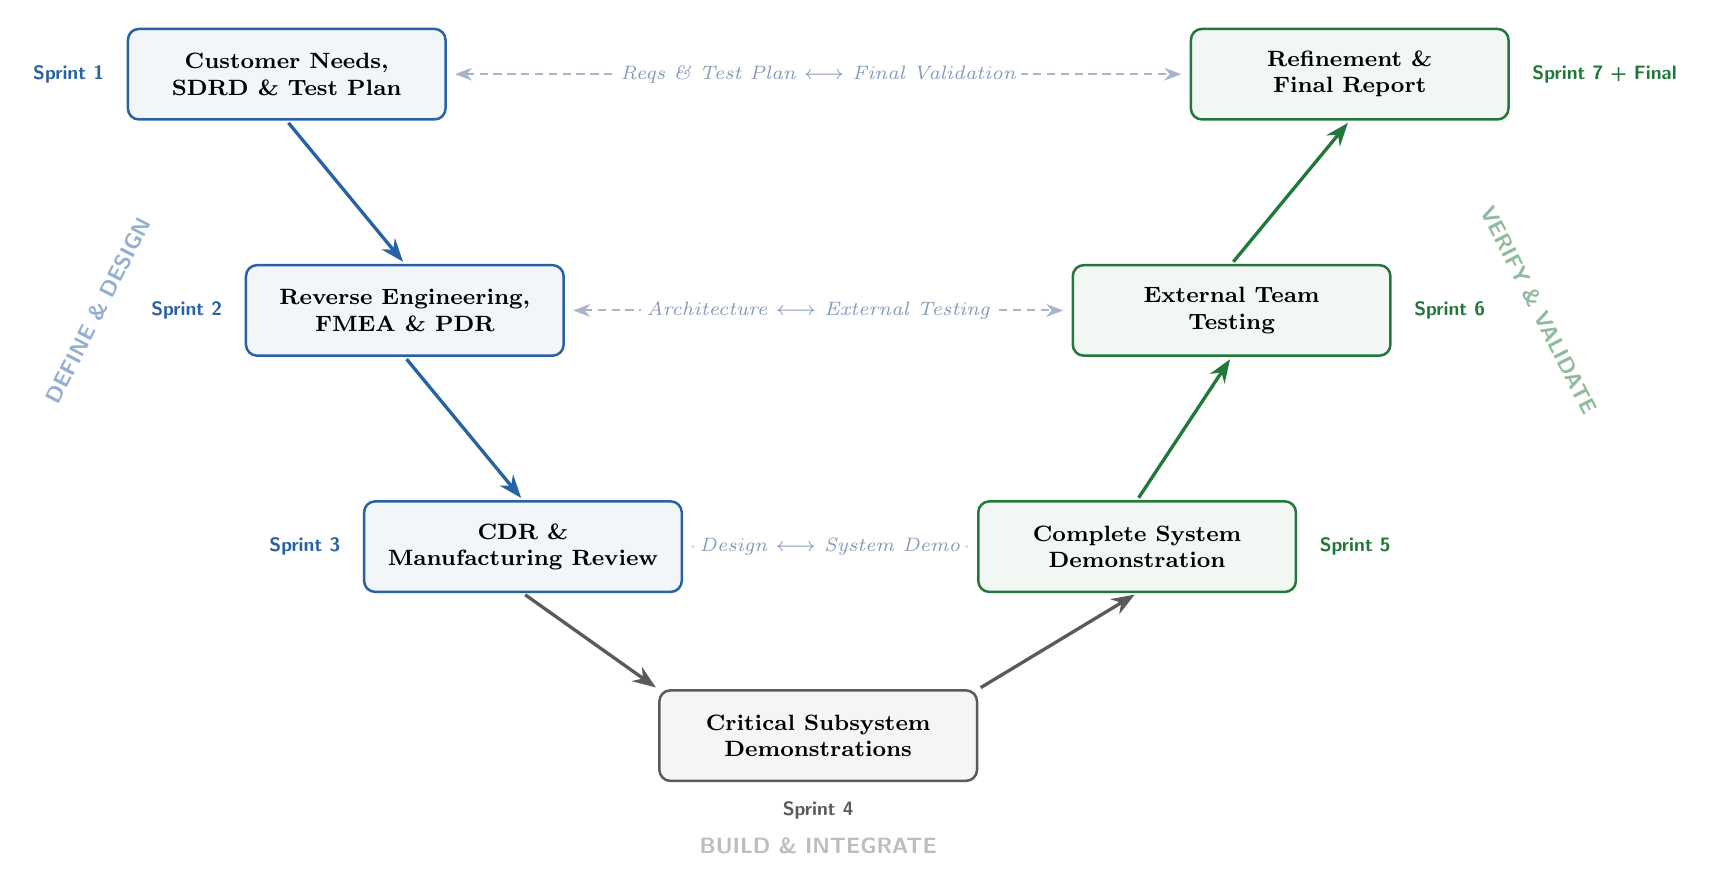
\begin{tikzpicture}[
    >=Stealth,
    % --- Node styles ---
    defblock/.style={
        rectangle, rounded corners=4pt, draw=vdefine, fill=vdefine!6,
        text width=3.8cm, minimum height=1.15cm, align=center,
        font=\footnotesize\bfseries, line width=0.9pt
    },
    verblock/.style={
        rectangle, rounded corners=4pt, draw=vverify, fill=vverify!6,
        text width=3.8cm, minimum height=1.15cm, align=center,
        font=\footnotesize\bfseries, line width=0.9pt
    },
    botblock/.style={
        rectangle, rounded corners=4pt, draw=vbuild, fill=vbuild!6,
        text width=3.8cm, minimum height=1.15cm, align=center,
        font=\footnotesize\bfseries, line width=0.9pt
    },
    slabel/.style={
        font=\scriptsize\sffamily\bfseries, color=#1,
        inner sep=2pt, fill=white, rounded corners=1pt
    },
    trace/.style={
        densely dashed, minesblue!40, line width=0.7pt, <->,
        shorten <=3pt, shorten >=3pt
    },
    tracelabel/.style={
        font=\scriptsize\itshape, text=minesblue!55, fill=white,
        inner sep=2pt, rounded corners=1pt
    },
    flow/.style={
        ->, line width=1.2pt, color=#1, shorten <=1pt, shorten >=1pt
    }
]

% === Symmetric V — labels on outer edges to keep arrow paths clear ===

% --- LEFT ARM (Define & Design) ---
\node[defblock] (L1) at (0, 0)      {Customer Needs,\\SDRD \& Test Plan};
\node[defblock] (L2) at (1.5, -3.0) {Reverse Engineering,\\FMEA \& PDR};
\node[defblock] (L3) at (3.0, -6.0) {CDR \&\\Manufacturing Review};

% --- BOTTOM VERTEX (Build & Integrate) ---
\node[botblock] (B)  at (6.75, -8.4)  {Critical Subsystem\\Demonstrations};

% --- RIGHT ARM (Verify & Validate) ---
\node[verblock] (R3) at (10.8, -6.0)  {Complete System\\Demonstration};
\node[verblock] (R2) at (12.0, -3.0)  {External Team\\Testing};
\node[verblock] (R1) at (13.5, 0)     {Refinement \&\\Final Report};

% --- Sprint labels: LEFT side for left arm, RIGHT side for right arm ---
\node[slabel=vdefine, left=6pt of L1]  {Sprint 1};
\node[slabel=vdefine, left=6pt of L2]  {Sprint 2};
\node[slabel=vdefine, left=6pt of L3]  {Sprint 3};
\node[slabel=vbuild,  below=5pt of B]  {Sprint 4};
\node[slabel=vverify, right=6pt of R3] {Sprint 5};
\node[slabel=vverify, right=6pt of R2] {Sprint 6};
\node[slabel=vverify, right=6pt of R1] {Sprint 7 + Final};

% --- Flow arrows (clean vertical paths — no labels in the way) ---
\draw[flow=vdefine] (L1.south) -- (L2.north);
\draw[flow=vdefine] (L2.south) -- (L3.north);
\draw[flow=vbuild]  (L3.south) -- (B.north west);
\draw[flow=vbuild]  (B.north east) -- (R3.south);
\draw[flow=vverify] (R3.north) -- (R2.south);
\draw[flow=vverify] (R2.north) -- (R1.south);

% --- Horizontal traceability arrows (same y-level matched pairs) ---
\draw[trace] (L1.east) -- node[tracelabel, midway] 
    {Reqs \& Test Plan $\longleftrightarrow$ Final Validation} (R1.west);

\draw[trace] (L2.east) -- node[tracelabel, midway] 
    {Architecture $\longleftrightarrow$ External Testing} (R2.west);

\draw[trace] (L3.east) -- node[tracelabel, midway] 
    {Design $\longleftrightarrow$ System Demo} (R3.west);

% --- Arm labels — pushed well outside the V to avoid crossing arrows ---
\node[rotate=63, font=\footnotesize\sffamily\bfseries, color=vdefine!50]
    at (-2.4, -3.0) {DEFINE \& DESIGN};
\node[rotate=-63, font=\footnotesize\sffamily\bfseries, color=vverify!50]
    at (15.9, -3.0) {VERIFY \& VALIDATE};

% --- Bottom label ---
\node[font=\footnotesize\sffamily\bfseries, color=vbuild!40]
    at (6.75, -9.8) {BUILD \& INTEGRATE};

\end{tikzpicture}%
}% end resizebox
\caption{The MEGN 301 design project mapped onto the systems engineering V-model. Matched pairs sit at the same level: Sprint~1 requirements define the success criteria verified in the Sprint~7 final report; Sprint~2 architecture decisions are validated through Sprint~6 external testing; Sprint~3 detailed designs are verified by Sprint~5 system demonstrations. Sprint~4 sits at the vertex where design transitions to integration.}
\label{fig:vmodel}
\end{figure}

%=============================================================================
\section{Sprint 1 -- Market Analysis, SDRD, and Test Plan}
%=============================================================================

\begin{priorities}
\begin{enumerate}[leftmargin=*, itemsep=1pt, topsep=0pt]
    \item Write testable, quantified requirements---everything downstream depends on this.
    \item Draft the test plan \textit{in parallel} with the SDRD, not after.
    \item Use the market analysis to make at least one concrete design decision.
\end{enumerate}
\end{priorities}

\begin{protip}
\textbf{Map out the semester calendar now.} Two short weeks hit early: \textbf{Career Day (Feb.~3)} cancels your Tuesday class during Sprint~2, and \textbf{Presidents' Day Break (Feb.~17)} cancels Tuesday during the Sprint~2/3 transition. \textbf{Spring Break (Mar.~24--28)} shuts down campus---including shipping and receiving, the machine shop, and all labs. If a component fails during Sprint~4 demos (Mar.~10--12) and you need a replacement, you must order it \textit{before} break. Build your sprint timelines around these gaps at your very first team meeting. Also note: \textbf{more than 3 unexcused absences results in automatic failure}. Being physically present but not participating (playing games, watching videos, working on other classes) counts as absent.
\end{protip}

\subsection{Market Analysis}

\begin{faqbox}[Q: Where should I look for competing products?]
Start with Amazon, specialty retailers, and Kickstarter/Indiegogo for consumer products in your space. Do not limit yourself to exact matches---look for products that solve the same underlying \textit{problem}, even if the form factor is different. For example, if your project is the Smart Canine Nutrition Station, look at automatic pet feeders, smart pet bowls, and pet health monitoring systems.
\end{faqbox}

\begin{faqbox}[Q: What makes a good pros/cons table?]
Focus on attributes the \textit{customer} cares about---not just specs. ``Uses a 12-bit ADC'' is an engineering detail; ``accurately portions food within $\pm$5 grams'' is something a pet owner cares about. Good categories include price, ease of setup, reliability (check those 1-star reviews!), power source flexibility, app quality, and compatibility with existing products.
\end{faqbox}

\begin{warnbox}
Do not treat the market analysis as a check-the-box exercise. The whole point is to identify a gap or weakness in what is currently available and use that insight to \textit{differentiate} your design. If your market analysis does not change at least one thing about how you think about your project, you probably did not dig deep enough.
\end{warnbox}

\begin{protip}
\textbf{Use the Five-Element Problem Statement Framework.} Before you jump to solutions, make sure you can clearly articulate: (1)~\textbf{WHO} experiences the problem, (2)~\textbf{WHAT} is the measurable gap between the current and desired state, (3)~\textbf{WHERE} does the problem occur (physical/operational context), (4)~\textbf{WHY IT MATTERS} (cost, safety, health consequences), and (5)~\textbf{CONSTRAINTS} that limit the solution (budget, schedule, regulations). If your problem statement implies only one possible solution, you have jumped into the solution space too early. A good problem statement lets someone propose a fundamentally different approach. See the Master Reference Document, Chapter~1, for detailed examples.
\end{protip}

\subsection{Patent Search}

\begin{faqbox}[Q: I have never read a patent before. What do I actually need to look at?]
Three things: (1) the \textbf{filing/grant date} (patents expire after 20 years from filing, so anything filed before roughly 2006 is now public domain), (2) the \textbf{abstract} (a quick summary to see if it is relevant), and (3) the \textbf{claims} (usually at the very end---these define exactly what is legally protected). You do \textit{not} need to read the entire patent specification.
\end{faqbox}

\begin{tipbox}
Use Google Patents (\url{https://patents.google.com/}) and try multiple search terms. If your first search returns thousands of irrelevant results, narrow it with more specific terminology. Combining a broad term with a functional term often works well, e.g., ``automatic pet feeder dispensing mechanism'' rather than just ``pet feeder.''
\end{tipbox}

\subsection{Customer Needs (AI Persona Interviews)}

\begin{faqbox}[Q: How do I get useful information out of an AI-generated persona?]
Treat the AI persona like a real customer interview. Ask open-ended questions first (``Walk me through a typical morning with your dog's feeding routine'') before drilling into specifics. Avoid leading questions like ``Wouldn't it be great if the feeder had an app?'' Instead, ask ``How do you currently keep track of feeding times?'' Let the persona reveal the pain points organically.
\end{faqbox}

\begin{protip}
Create three personas that represent \textit{different} user segments, not three variations of the same person. For example, for the Medication Assistant: a caregiver managing multiple patients, an independent elderly person living alone, and a busy parent managing a child's medication. Different personas surface different needs.
\end{protip}

\begin{warnbox}
\textbf{GenAI Policy Boundary:} The AI persona interview assignment \textit{requires} you to use Gemini Pro (via your Mines email). However, this is the \textbf{only} approved GenAI use in the course. You may \textit{not} use GenAI to write your SDRD requirements, generate your test plan, compose your FMEA, write your retrospectives, or produce your reports. GenAI is the \textit{subject} of this exercise---it is not your co-author. Any unapproved use of GenAI technologies is an honor code violation.
\end{warnbox}

\subsection{System Design Requirements Document (SDRD)}

\begin{faqbox}[Q: What is the difference between an objective and a requirement?]
An \textbf{objective} is qualitative---it describes \textit{what} the system should do or be. A \textbf{requirement} is quantitative---it specifies a measurable threshold that proves the objective is met. For example, Objective: ``The system shall dispense food accurately.'' Requirement: ``The system shall dispense the user-specified amount of food within $\pm$10\% by weight.''
\end{faqbox}

\begin{faqbox}[Q: How do I know if a requirement is well-written?]
Apply the ``stranger test'': could someone who has never seen your project read the requirement and know \textit{exactly} what to measure, how to measure it, and what constitutes a pass or fail? If the answer is no, the requirement needs work. Every requirement must be clear, quantifiable, and testable. To illustrate, here is the same requirement at three levels of quality:

\begin{center}
\renewcommand{\arraystretch}{1.3}
\begin{tabularx}{0.95\textwidth}{>{\bfseries\color{warnred}}c >{\raggedright\arraybackslash}X}
\toprule
\textbf{Level} & \textbf{Requirement} \\
\midrule
\textcolor{warnred}{Bad} & ``The system shall be durable.'' \\
\textcolor{minesgold!80!black}{Better} & ``The system shall survive a drop.'' \\
\textcolor{tipgreen}{Best} & ``The system shall maintain full mechanical and electrical functionality after a 1-meter drop onto a concrete surface, verified by executing the full test suite immediately after the drop.'' \\
\bottomrule
\end{tabularx}
\end{center}

\noindent The ``Bad'' version is untestable. ``Better'' adds a physical event but leaves out the height, surface, and acceptance criteria. ``Best'' specifies everything a tester needs: drop height, surface material, and a concrete pass/fail procedure. Aim for ``Best'' on every requirement.
\end{faqbox}

\begin{warnbox}
Vague requirements like ``the system shall be easy to use'' or ``the system shall be reliable'' are the number one source of problems later in the semester. They are impossible to test, which means you cannot demonstrate that your prototype meets them. Rewrite them: ``A first-time user shall be able to complete the setup process in under 5 minutes without external assistance'' is testable.
\end{warnbox}

\begin{tipbox}
Write your requirements and your test plan \textit{at the same time}. If you cannot immediately envision how you would test a requirement, it is either too vague or unmeasurable. This back-and-forth process naturally produces better requirements.
\end{tipbox}

\begin{protip}
\textbf{Prioritize requirements using MoSCoW.} Not all requirements are equally critical. Classify each as: \textbf{Must} (system fails without it---becomes a SHALL requirement), \textbf{Should} (important but system works without it---becomes a SHOULD goal), \textbf{Could} (nice-to-have, pursue if budget allows), or \textbf{Won't} (explicitly excluded from this version). This prevents scope creep and helps your team focus on the requirements that matter most when time gets tight. See the Master Reference Document, Chapter~1, for how MoSCoW ties into stakeholder needs management.
\end{protip}

\subsection{Test Plan}

\begin{faqbox}[Q: How detailed does the test plan need to be?]
Detailed enough that a team who has \textit{never seen your project} can execute every test. Remember, in Sprint~6 an external team will be running your test plan. If they have to guess what you meant, you will get ambiguous results. Specify equipment needed, step-by-step procedures, pass/fail criteria, and expected duration for each test.
\end{faqbox}

\begin{faqbox}[Q: Does every single SDRD requirement need a corresponding test?]
Yes. If a requirement exists in your SDRD but has no test, then you have no way to verify that requirement is met. Either write a test for it or reconsider whether it should be in the SDRD. There should be a one-to-one (or many-to-one) mapping from tests to requirements.
\end{faqbox}

\begin{tipbox}
\textbf{Know the four verification methods (TAID).} Not every requirement is verified by running a physical test. The four methods are: \textbf{Test} (measure performance under controlled conditions), \textbf{Analysis} (verify by calculation, simulation, or modeling), \textbf{Inspection} (verify by visual or dimensional examination), and \textbf{Demonstration} (verify by operating the system through its use cases). Assign a verification method to each requirement when you write it. Most of your requirements will use Test or Demonstration, but some (e.g., material compliance, dimensional tolerances) may be verified by Inspection or Analysis. See the Master Reference Document, Chapter~4, for detailed guidance on TAID and writing test procedures.
\end{tipbox}

\subsection{Sprint Retrospective}

\begin{faqbox}[Q: What is the point of the retrospective?]
The retrospective is not busywork---it is a structured opportunity to improve your team's process. Be honest about what went well, what did not, and what you will change. The best teams use retrospectives to catch problems early (e.g., unbalanced workloads, communication gaps, unclear task ownership) before they become crises.
\end{faqbox}

%=============================================================================
\section{Sprint 2 -- Preliminary Design Review (PDR)}
%=============================================================================

\begin{priorities}
\begin{enumerate}[leftmargin=*, itemsep=1pt, topsep=0pt]
    \item Thoroughly reverse engineer the COTS product---especially its electrical interfaces.
    \item Complete an honest FMEA; do not downplay severity to look ``clean.''
    \item Weight your decision matrix criteria \textit{before} scoring alternatives.
\end{enumerate}
\end{priorities}

\begin{protip}
\textbf{Start with functional decomposition before jumping to components.} Before picking sensors, microcontrollers, or actuators, list the \textit{functions} your system must perform using verb-noun pairs: Sense Temperature, Dispense Food, Filter Air, etc. Then break each function into sub-functions. This separates \textit{what} the system must do from \textit{how} it does it, and it directly feeds your trade study. A morphological chart---listing functions as rows and 3--5 implementation options as columns---is the most powerful way to systematically generate meaningfully different design concepts. See the Master Reference Document, Chapters~2--3, for worked examples using the GreenShield case study.
\end{protip}

\subsection{Reverse Engineering}

\begin{faqbox}[Q: What am I actually looking for when I reverse engineer the COTS product?]
You are trying to answer: ``What constraints does this existing product impose on my add-on design?'' Look for mounting points, electrical interfaces (voltage, current, connector types), physical dimensions and tolerances, material properties, and any features that could either help or hinder your integration. Document everything with photos and measurements.
\end{faqbox}

\begin{protip}
Measure twice (or three times). Tolerances on consumer products can be surprisingly loose. If you are designing a mechanical interface, build in adjustability or compliance rather than relying on a single measurement from one unit.
\end{protip}

\begin{warnbox}
Explicitly document the \textbf{connectors and power draw} of the COTS product during reverse engineering. One of the most common integration failures occurs when an add-on system pulls more current than the parent product's power supply can handle, or when the team orders a mating connector with the wrong pitch (e.g., 2.0\,mm vs.\ 2.54\,mm JST headers). Record connector type, pin count, pitch, voltage, and rated/measured current draw. This information is critical for your CDR and will prevent expensive, time-consuming mistakes in Sprints~3--4.
\end{warnbox}

\subsection{Failure Modes and Effects Analysis (FMEA)}

\begin{faqbox}[Q: How do I identify failure modes I have not thought of yet?]
Systematically walk through every component and every interface in your system and ask: ``What happens if this breaks, jams, shorts, overheats, receives the wrong input, or loses power?'' Also consider misuse scenarios---what if the user does something unexpected? The USCSB ExxonMobil video assigned in this sprint is an excellent example of how overlooked failure modes cascade into catastrophic outcomes.
\end{faqbox}

\begin{warnbox}
Do not assign uniformly low severity or occurrence ratings to make your FMEA look ``clean.'' An FMEA with no high-risk items is almost certainly an FMEA that was not done thoroughly. Instructors will see through this immediately. The value of the FMEA is in \textit{finding} the scary stuff so you can address it in your design.
\end{warnbox}

\begin{tipbox}
\textbf{Score the FMEA using three independent scales.} Each failure mode gets rated on Severity (how bad if it happens, 1--10), Occurrence (how likely, 1--10), and Detection (how likely the failure goes unnoticed, 1--10). Multiply them to get the Risk Priority Number: $\text{RPN} = S \times O \times D$. Failure modes with RPN $\geq 100$ generally need corrective action in your design. A high-severity, low-occurrence, hard-to-detect failure (e.g., temperature sensor reading high so frost is not detected---$S=9, O=3, D=5, \text{RPN}=135$) demands more attention than an obvious, low-impact failure. Prioritize your design resources based on RPN, not gut feeling.
\end{tipbox}

\begin{protip}
\textbf{Think about all six types of interfaces during your FMEA.} Failures cluster at interfaces, not inside components. The six interface categories are: electrical (voltage, protocol, grounding), mechanical (mounting, tolerances, alignment), thermal (heat paths, contact resistance, component overheating), software/data (APIs, data format, timing), fluid (fittings, pressure, seal compatibility), and human (display visibility, control layout, error prevention). Walk through each interface in your system and ask what happens when each one fails.
\end{protip}

\subsection{PDR Report and Decision Matrix}

\begin{faqbox}[Q: How many design alternatives should we consider in the trade study?]
At minimum, you should have three meaningfully different concepts. ``Meaningfully different'' means different architectures or approaches, not minor variations of the same idea (e.g., ``same design but in blue'' does not count). The decision matrix should use weighted criteria that trace back to your customer needs and SDRD objectives.
\end{faqbox}

\begin{tipbox}
When building your decision matrix, weight the criteria \textit{before} scoring the alternatives. This prevents the common bias of adjusting weights after the fact to justify the concept you already wanted to build.
\end{tipbox}

\begin{protip}
\textbf{Run a sensitivity analysis on your decision matrix.} After scoring, vary each weight by $\pm$0.05 and check whether the winning concept changes. For instance, if Concept~A beats Concept~B by only 0.05 points, and shifting the ``cost'' weight by 10\% makes Concept~B the winner, your decision is not robust---you need better data on that criterion or should prototype both options. A margin of less than 5\% between the top two concepts demands additional investigation, not a hasty commitment. Also ensure every candidate is a legitimate contender: including a deliberately weak ``straw man'' option to make your preferred concept win is a common pitfall that instructors spot immediately.
\end{protip}

\begin{faqbox}[Q: How do I know if my PDR package is ready?]
Apply the \textbf{PDR Litmus Test}: ``If a different engineering team read only our PDR package, could they independently arrive at the same concept selection and understand why it is the best choice?'' If the answer is yes, your PDR is defensible. If the answer requires ``well, they would also need to know that\ldots''---that missing information must be added to the package. Remember, PDR answers the question ``\textit{Should} this design work?'' Your deliverables must demonstrate that the problem is well-defined, the requirements are sound, and the selected concept is feasible.
\end{faqbox}

%=============================================================================
\section{Sprint 3 -- Critical Design Review (CDR)}
%=============================================================================

\begin{priorities}
\begin{enumerate}[leftmargin=*, itemsep=1pt, topsep=0pt]
    \item Submit purchase requests as early as possible---do not wait for the CDR deadline.
    \item Design polymer parts for injection molding, even though you are prototyping with 3D printing.
    \item Get every manufactured part reviewed by the appropriate resource \textit{before} fabrication.
\end{enumerate}
\end{priorities}

\subsection{CDR Report}

\begin{faqbox}[Q: What does ``everything someone would need to build your prototype'' actually mean?]
Imagine handing your CDR to a competent engineering team that has never met you. Could they purchase the correct components, fabricate every part, assemble the system, and load the software? If not, something is missing. This means complete CAD drawings with dimensions and tolerances, a full bill of materials with part numbers and vendors, wiring diagrams, software architecture descriptions, and assembly instructions.
\end{faqbox}

\begin{protip}
\textbf{Build a power budget spreadsheet before anything else.} List every component with its voltage rail, continuous current draw, and peak current draw. Sum the columns and add a 25\% margin. This single spreadsheet will tell you whether your power supply is adequate, what regulator stages you need, and where your thermal hotspots will be. Motor inrush is the number-one power supply problem: a motor rated at 2\,A running may draw 15\,A at startup. Size your supply for inrush, not steady state. See the Master Reference Document, the Power Architecture chapter, for design rules and the derating guideline: 20\% margin on power supplies, 25--50\% on motors, 25\% on pumps.
\end{protip}

\begin{warnbox}
\textbf{Separate your power and signal grounds.} Poor grounding is the most common cause of hard-to-diagnose intermittent failures in student projects---noisy sensor readings, MCU resets when a motor starts, dropped serial communication. Run motor power on dedicated ground wires back to the supply; never share ground paths between motors and sensitive electronics. Use star-point grounding: each subsystem gets its own ground conductor, and they all meet at one common point near the power supply. See the Master Reference Document, the Power Architecture chapter, for the three-ground-domain strategy (signal, power, safety earth).
\end{warnbox}

\begin{tipbox}
\textbf{Identify a ``Plan B'' component for every critical item.} For any single-source or sole-vendor component in your BoM, record a backup part number and vendor in a notes column. If your specialty sensor, MOSFET, or pump goes out of stock the week before CDR, you need to order the backup \textit{immediately}---not start a new search. This is especially important for projects with specialty components like the \textit{Sous Vide Supreme} (heating elements) and \textit{Sol-Mate Purification Pal} (solar charge controllers), where lead times can exceed two weeks.
\end{tipbox}

\subsection{Purchase Requests}

\begin{faqbox}[Q: When should we submit our purchase request?]
As early as possible. Do not wait until the CDR deadline. Shipping delays are real, and if a component arrives late, your build schedule slips. Identify long-lead-time items (specialty sensors, custom PCBs, specific actuators) early and flag them to your instructor. Have a backup vendor or component in mind for critical items.
\end{faqbox}

\begin{warnbox}
Only order from the approved vendor list. Unapproved vendors require a review and may be denied, which costs you time. Check the list before you fall in love with a component that is only available from a vendor not on the list.
\end{warnbox}

\begin{warnbox}
\textbf{The Spring Break Shipping Trap.} Spring Break begins March~24---campus shipping/receiving, the machine shop, and all lab facilities are \textbf{closed} that week. If a component fails during your Sprint~4 subsystem demo (around Mar.~10--12) and you need a replacement for the full system demo, you must order it \textit{immediately}---not after break. Plan your procurement so all critical components arrive before March~21. The same logic applies to 3D prints and machined parts: submit them early enough to allow for at least one iteration before campus shuts down.
\end{warnbox}

\subsection{Manufacturing Design Review}

\begin{faqbox}[Q: Why do polymer components need to be designed for injection molding?]
Even though your prototype will likely be 3D printed, designing for injection molding teaches you to think about manufacturability at scale. This means uniform wall thickness, draft angles, avoiding undercuts, and proper rib and boss design. The white paper provided on Canvas covers these principles in detail. This is a skill that will serve you in every future design role.
\end{faqbox}

\begin{faqbox}[Q: Which 3D printing process should I choose?]
Use \textbf{filament (FDM) printing} for larger structural components where surface finish is less critical. Use \textbf{resin (SLA) printing} for small, detailed parts that require tighter tolerances or smoother surfaces. Refer to Appendix A of the project document for resin printer settings. Get your designs reviewed early---the machine shop assistants, Prof.\ Blood, and the Master TAs are all available to help.
\end{faqbox}

\begin{protip}
\textbf{Use heat-set inserts or captive nuts for any structural fastening into 3D-printed parts.} Students frequently try to tap threads directly into FDM prints or rely on superglue for structural joints---both approaches fail under load and vibration, often catastrophically during a live demo. Brass heat-set inserts (installed with a soldering iron) create strong, reusable M3/M4 threads in printed parts for pennies each. Design the appropriately sized pilot hole into your CAD model from the start. This is a small investment that prevents mid-demo disasters.
\end{protip}

\begin{tipbox}
Complete your Order of Operations sheet \textit{before} walking into the machine shop. This is required for machined parts and is also just good practice---it forces you to think through the fabrication sequence, which often reveals design issues before you waste material.
\end{tipbox}

\begin{protip}
\textbf{Choose your resin strategically to save budget.} The campus resin printers support two materials at very different price points: Elegoo ABS-Like at \$15/kg and Siraya Tech Blu Nylon-Like at \$38/kg (see Appendix~A of the project document for settings). Use the cheaper ABS-like resin for basic structural enclosures, brackets, and cosmetic parts. Reserve the Nylon-like resin only for parts requiring high toughness, wear resistance, or repeated flexure---gears, snap-fit clips, or living hinges. A single strategic resin choice can save \$20--40 of your project budget.
\end{protip}

\begin{tipbox}
\textbf{Document every electrical connection and every software flow \textit{now}, not later.} Your CDR should include a wiring diagram showing every component, wire color, gauge, connector part number, and pinout, plus a programming flowchart showing your main loop, state machine transitions, sensor reads, actuator control logic, and error handling. These diagrams are the electrical and software equivalents of your CAD drawings---without them, no one (including your future self at 10~PM during Sprint~5) can debug your system. See the Master Reference Document, Chapter~3, for wiring diagram and flowchart best practices.
\end{tipbox}

\begin{protip}
\textbf{Decide early: dev boards or custom PCB?} Use development boards (Arduino, ESP32 DevKit, sensor breakouts) when your circuit is straightforward, form factor is not critical, the timeline is tight, or the design is still evolving. Use a custom PCB when a specific enclosure size is required, noise-sensitive analog signals demand a ground plane, or you need clean cable routing and high reliability. A well-wired dev board that meets requirements is superior to a custom PCB that delays the project. If you do go custom, the total timeline from design start to working board is 4--6 weeks (design, order from JLCPCB/PCBWay, ship, solder, debug), so your design must be frozen at CDR. See the Master Reference Document, PCB Design chapter, for the complete workflow, layout rules, and fab house options.
\end{protip}

\begin{warnbox}
\textbf{ESP32 GPIO gotchas that will cost you a day of debugging.} If your project uses an ESP32 (the recommended MCU for this course), memorize these before assigning pins: \textbf{GPIO 6--11} are connected to internal flash---do not use them for anything or the board will not boot. \textbf{GPIO 34--39} are input-only---no output capability, no internal pull-ups. \textbf{ADC2 is disabled when Wi-Fi is active}---use only ADC1 channels (GPIO 32--39) for analog readings in any project that uses Wi-Fi. \textbf{3.3\,V logic only}---use level shifters for 5\,V sensors or actuators. \textbf{Boot pins (0, 2, 12, 15)} can prevent startup if pulled to unexpected levels. Safe GPIOs for general use: 4, 13, 14, 16--19, 21--23, 25--27, 32, 33. See the Master Reference Document, Microcontrollers chapter, for the complete pin map and power mode details.
\end{warnbox}

\begin{faqbox}[Q: How do I know if my CDR package is ready?]
Apply the \textbf{CDR Litmus Test}: ``If I handed this CDR package to a competent technician who has never seen this project, could they build the prototype from these documents alone?'' If the BOM is complete, the drawings are dimensioned, the wiring diagram is unambiguous, and the assembly sequence is clear---your CDR is ready. If the answer requires ``well, they would also need to know that\ldots''---that missing information must be added. CDR answers ``\textit{Will} this design work?''---it is the point of no return where you commit resources to procurement and fabrication.
\end{faqbox}

\begin{tipbox}
\textbf{Save a ``CDR baseline'' snapshot of all your documents.} After CDR, you will compare your as-designed BOM, budget, and drawings against the as-built reality at FDR. Create a frozen copy of your CDR package (BOM, CAD, wiring diagrams, firmware version, budget) before you start building. This makes the as-designed vs.\ as-built comparison in your final report straightforward instead of a painful reconstruction exercise.
\end{tipbox}

%=============================================================================
\section{Sprint 4 -- Critical Subsystem Demonstrations}
%=============================================================================

\begin{priorities}
\begin{enumerate}[leftmargin=*, itemsep=1pt, topsep=0pt]
    \item Get your demo proposal approved \textit{before} this sprint begins.
    \item Choose the two highest-risk subsystems, not the easiest ones.
    \item Record a narrated video and verify the link works in incognito mode.
\end{enumerate}
\end{priorities}

\begin{faqbox}[Q: How do I choose which two subsystems to demonstrate?]
Pick the two subsystems that represent the highest technical risk in your design. These are the parts you are least certain will work, or the parts that, if they fail, would require the biggest redesign. The purpose of this sprint is to retire risk early. Demonstrating something you are already confident about wastes this opportunity.
\end{faqbox}

\begin{faqbox}[Q: What if my demo does not fully meet the proposed goals?]
That is okay---this is expected to happen sometimes, and it is why the demo report asks you to document what modifications are needed. The important thing is to (1) clearly state what worked and what did not, (2) provide specific performance data (not just ``it kind of worked''), and (3) outline a concrete plan to address the gaps before the full system demo.
\end{faqbox}

\begin{warnbox}
Get your demo proposal approved by your instructor \textit{before} Sprint 4 begins. If you wait, you risk demonstrating something your instructor considers too easy or not aligned with your project's critical path, and you will have to redo it.
\end{warnbox}

\begin{protip}
When you record your demonstration video, narrate what you are doing and what the expected vs.\ actual results are. A silent video of a blinking LED tells the viewer nothing. Also, verify your video link is accessible by opening it in an incognito/private browser window. Unviewable links may receive a zero.
\end{protip}

\begin{warnbox}
\textbf{Never ``big-bang'' integrate.} Assembling every component at once and powering on is the fastest route to an undebuggable system. Instead, use bottom-up integration: verify each component individually, then add \textbf{one new element at a time} and test after each addition. When something breaks, the last thing you added (or its interface) is the prime suspect. For most electromechanical projects, a good integration sequence is: (1)~power supply first (everything depends on it), (2)~controller (the central hub), (3)~sensors (simplest interfaces), (4)~actuators (highest power, most failure modes), (5)~communication (can be tested last since it is not needed for core function).
\end{warnbox}

\begin{tipbox}
\textbf{If you designed a custom PCB, follow the bring-up protocol before connecting it to anything.} (1)~Visual inspection under magnification for solder bridges, cold joints, and wrong-orientation parts. (2)~Continuity check with a multimeter---confirm no shorts between VCC and GND. (3)~Current-limited power: set your bench supply to 50\,mA limit and apply voltage. (4)~Measure every power rail with a multimeter. (5)~Smoke test: increase current to operating level, monitor for 60 seconds. (6)~Load firmware and test basic I/O. Skipping this sequence and plugging a freshly soldered board straight into your system is how you destroy both the board and the system in one step. See the Master Reference Document, PCB Design chapter, for the full protocol.
\end{tipbox}

\begin{tipbox}
\textbf{Run multiple trials, not just one.} A subsystem that works once under ideal bench conditions may fail intermittently under real operating conditions. For each demonstration goal, run at least 3 trials (5 is better). Report the mean, standard deviation, and range of your measurements---for example, for a temperature sensor demo, report: ``Mean error = $0.32\,^{\circ}\text{C}$, $\sigma = 0.04\,^{\circ}\text{C}$, range $0.26$--$0.41\,^{\circ}\text{C}$, $n = 5$ trials at each of three test points,'' not just ``it read the right temperature.'' Test at boundary conditions, not just room temperature on a benchtop. A result of ``PASS with 36\% margin'' is far more convincing---and useful---than a bare ``PASS.''
\end{tipbox}

%=============================================================================
\section{Sprint 5 -- Complete System Demonstration}
%=============================================================================

\begin{priorities}
\begin{enumerate}[leftmargin=*, itemsep=1pt, topsep=0pt]
    \item Demonstrate end-to-end functionality from the user's perspective.
    \item Update the BoM with actual costs and a labor estimate.
    \item Finalize the test plan so it is ready for the external team---this is your last chance to fix ambiguities.
\end{enumerate}
\end{priorities}

\begin{faqbox}[Q: What should I focus on for the in-class system demo?]
Show that your system works \textit{end-to-end} as a user would experience it. Start with the user powering on the system, walk through the primary use case, and demonstrate key requirements being met. If something is not working, be upfront about it. Instructors value honesty and a clear understanding of what went wrong far more than a polished demo that hides problems.
\end{faqbox}

\begin{faqbox}[Q: My design has changed a lot since the CDR. Is that a problem?]
Not at all---design iteration is expected and encouraged. What matters is that you \textit{document} the changes: what changed, when it changed, and why. Part A of the Complete System Demo Report specifically asks for this. A well-documented design evolution shows engineering maturity.
\end{faqbox}

\begin{protip}
\textbf{When debugging integration failures, follow a five-step process.} (1)~\textbf{Reproduce}: make the failure happen reliably and note the exact conditions. A failure you cannot reproduce is a failure you cannot fix. (2)~\textbf{Isolate}: disconnect modules one at a time until the failure stops---the last module disconnected is the prime suspect. (3)~\textbf{Characterize}: measure signals at the interface with an oscilloscope or multimeter and compare to your ICD specifications. (4)~\textbf{Root-cause}: determine whether the problem is hardware, software, or an interface specification error. (5)~\textbf{Fix and regression-test}: implement the fix, verify it resolves the original failure, then \textit{re-run all previously passed tests} to confirm the fix did not break anything else. \textbf{Change ONE variable at a time.} If you swap firmware and a component simultaneously, you will not know which change fixed it---and the other may have introduced a new latent defect.
\end{protip}

\begin{tipbox}
Use this sprint to finalize your test plan for the external team. Read through every test procedure as if you have never seen the project before. If any step is ambiguous, fix it now. You will not be in the room when the external team runs your tests.
\end{tipbox}

\begin{warnbox}
Do not forget to update your Bill of Materials (Part B) with actual costs, including any components you ended up not using or had to reorder. Also include a labor estimate---this is easy to overlook but is required.
\end{warnbox}

\begin{protip}
\textbf{Build a Verification Cross-Reference Matrix (VCRM) before the system demo.} The VCRM is a simple table linking each requirement to its verification method, test procedure ID, and current status (Open, Verified, Failed, Waived). By Sprint~5, you should be able to fill in most of this table. It becomes the single artifact that tells the complete project story at your final review, and it makes writing the final report dramatically easier. See the Master Reference Document, Chapter~4, for a worked VCRM example at PDR, CDR, and FDR milestones.
\end{protip}

\begin{tipbox}
\textbf{When a test fails, investigate root causes in order.} Three possible sources, checked in this sequence: (1)~Is the \textit{test} wrong? (procedure error, miscalibrated equipment, incorrect setup), (2)~Is the \textit{implementation} wrong? (the most common cause---a component, connection, or code issue), (3)~Is the \textit{requirement} wrong? (overly conservative or based on flawed assumptions). Only consider changing a requirement after ruling out the first two, and any requirement change must be formally documented with rationale. Never silently adjust a requirement to make a failed test ``pass.''
\end{tipbox}

%=============================================================================
\section{Sprint 6 -- External Team Testing}
%=============================================================================

\begin{priorities}
\begin{enumerate}[leftmargin=*, itemsep=1pt, topsep=0pt]
    \item Hand off a clean, well-labeled prototype with a complete test plan.
    \item Observe the ``Silent Observer'' rule: do not coach the testing team.
    \item When \textit{you} are the testing team, be thorough and professional.
\end{enumerate}
\end{priorities}

\begin{faqbox}[Q: What happens during external team testing?]
Another team will receive your prototype and your test plan, and they will execute your tests and document the results. You will \textit{not} be present to explain anything. This is the ultimate test of your documentation quality. Every ambiguity, missing step, or unclear pass/fail criterion in your test plan will surface here.
\end{faqbox}

\begin{tipbox}
\textbf{Prepare a handoff package, not just a prototype.} Before handing your system to the external team, prepare: (1)~a one-page quick-start guide with numbered steps and photos showing how to power on, configure, and operate the system, (2)~all required test equipment, cables, and fixtures laid out and labeled, (3)~clear photographs of the correct system configuration for each test, (4)~any safety precautions highlighted prominently, and (5)~your test plan reviewed one final time as if you have never seen the project. External testing typically reveals three categories of problems: procedure ambiguities (``connect the sensor'' without specifying which port), missing preconditions (the system needs 5 minutes of warm-up but the procedure says nothing about it), and actual system defects that your team never encountered because they operate the system differently.
\end{tipbox}

\begin{warnbox}
\textbf{The ``Silent Observer'' Rule:} During external testing, the designing team must remain \textbf{completely silent}. Do not coach, correct, hint, or demonstrate. If the testing team is struggling with a step, that is data---it means your documentation needs improvement. The moment someone says ``Oh, you just need to press it like this,'' you have invalidated the test of your documentation. Resist the urge. Let the test plan speak for itself. This is one of the most valuable learning experiences in the entire course.
\end{warnbox}

\begin{faqbox}[Q: What if the external team breaks something or does a test wrong?]
This is a real-world scenario---products must survive being used by people who did not design them. If a test is performed incorrectly, it likely means your test procedure was unclear. Use this feedback constructively. If something physically breaks, document it and address it in Sprint~7.
\end{faqbox}

\begin{protip}
When you are the \textit{testing} team for another group, be thorough and fair. Your primary goal is not to make the other team look bad---it is to provide honest, constructive feedback that helps them improve. Document everything that is ambiguous or unclear in the test plan; that feedback is a gift to the design team. The quality of your external testing report reflects your own engineering professionalism, and your teammates will return the favor. This is also an opportunity to see how another team approached a different design problem---you will learn things that make you a better engineer.
\end{protip}

%=============================================================================
\section{Sprint 7 -- Prototype Refinement and Retesting}
%=============================================================================

\begin{priorities}
\begin{enumerate}[leftmargin=*, itemsep=1pt, topsep=0pt]
    \item Fix every issue identified in external testing, prioritized by impact on core requirements.
    \item Re-test every fix before the final presentation.
    \item Begin drafting the final report and presentation---do not treat this sprint as a break.
\end{enumerate}
\end{priorities}

\begin{faqbox}[Q: There are no formal submissions for Sprint~7. What should I be doing?]
Three things: (1) address every issue identified during external team testing, (2) prepare your Final Design Oral Presentation, and (3) begin drafting your Final Design Report. This sprint is your buffer---use it wisely. Teams that treat Sprint~7 as a vacation week invariably produce weaker final deliverables.
\end{faqbox}

\begin{tipbox}
Prioritize fixes by impact. If external testing revealed that a core requirement failed, fix that first. Cosmetic issues and nice-to-haves come last. Make sure any fixes are re-tested before the final presentation. After each re-test, update your VCRM with the new results---this ensures the final VCRM is complete and current when you submit it as part of the FDR package.
\end{tipbox}

\begin{warnbox}
\textbf{Regression-test after every fix.} Any change to your system---firmware update, component swap, wiring modification---may break something that previously worked. After implementing each fix, re-run all tests affected by that change. A fix to the motor driver firmware might shift the EMI spectrum and corrupt your sensor ADC readings. Without regression testing, you may fix one problem and silently introduce three others. Use your VCRM to track which requirements need re-verification after each change.
\end{warnbox}

\begin{protip}
As you refine your prototype and prepare final deliverables, explicitly trace your results back to the course learning outcomes. Can you articulate which design decisions demonstrate your ability to define requirements, analyze trade-offs, manage risk, and verify performance? This traceability matters for course assessment, and it is exactly the kind of reflective practice that will distinguish you in Capstone, senior design, and industry.
\end{protip}

%=============================================================================
\section{Final Design Oral Presentation}
%=============================================================================

\begin{faqbox}[Q: How should we structure a 10-minute presentation?]
A recommended breakdown: introduction and problem statement (1 min), design requirements overview (1.5 min), design evolution from concept to final prototype (3 min), performance results and testing summary (2.5 min), future improvements and lessons learned (2 min). Practice with a timer. Ten minutes goes faster than you think, and you want to leave time for the 5-minute Q\&A.
\end{faqbox}

\begin{warnbox}
Do not try to cover everything. Your final report is where the details live. The presentation should tell a compelling \textit{story}: what problem did you solve, how did your design evolve, did it work, and what did you learn? Slides crammed with text and tiny font sizes are a sign that you are trying to say too much.
\end{warnbox}

\begin{protip}
Anticipate questions. Common ones include: ``Why did you choose this approach over the alternatives?'' ``What was your biggest design challenge?'' ``If you had another semester, what would you change?'' ``How much would this cost at production volume?'' Prepare concise answers to these in advance.
\end{protip}

%=============================================================================
\section{Final Design Report}
%=============================================================================

\begin{faqbox}[Q: How much of the final report can come from earlier sprint submissions?]
Much of it \textit{should} come from earlier sprints---that is by design. However, ``copy and paste from Sprint~3'' is not sufficient. You are expected to \textbf{revise and update} every section to reflect the final state of your project and address any issues identified in earlier sprint feedback. Treat this as a polished, standalone document that tells the complete story.
\end{faqbox}

\begin{faqbox}[Q: What goes in the appendix vs.\ the main body?]
The main body should contain your narrative, key results, and high-level design information. The appendix is for detailed supporting material: full CAD drawings, complete BoM, raw test data, detailed calculations, wiring diagrams, and software documentation. A good rule of thumb: if removing it would break the narrative flow of the main body, it belongs in the main body. If it is supporting evidence or reference material, it belongs in the appendix.
\end{faqbox}

\begin{faqbox}[Q: What should go in the ``Future Work'' and ``Hazards Discussion'' sections?]
For \textbf{Future Work}: think in terms of lifecycle. What refinements would bring the prototype to a production-ready product? Consider serviceability (can a technician access and replace the most failure-prone components?), maintenance planning (what are the wear items and their replacement intervals?), and a spare parts list with vendor part numbers. Thinking about Operations \& Maintenance is not an afterthought---it accounts for 50--70\% of a product's lifecycle cost. For the \textbf{Hazards Discussion}: revisit your FMEA with updated RPN scores. Discuss the highest-RPN failure modes you identified, what design changes you made to mitigate them, and whether those changes actually reduced the risk. Also address any new hazards discovered during prototyping and testing that were not in the original FMEA. See the Master Reference Document, Chapter~6, for the design-for-serviceability principles and FMECA methodology.
\end{faqbox}

\begin{faqbox}[Q: How honest should the ``Lessons Learned'' section be?]
Very. This section is not about making yourself look good---it is about demonstrating that you grew as engineers. The best lessons learned sections candidly discuss what went wrong, why it went wrong, and what the team would do differently. Instructors can tell the difference between generic filler and genuine reflection. Compare these two examples:

\begin{center}
\renewcommand{\arraystretch}{1.3}
\begin{tabularx}{0.95\textwidth}{>{\bfseries\color{warnred}}c >{\raggedright\arraybackslash}X}
\toprule
\textbf{Quality} & \textbf{Example} \\
\midrule
\textcolor{warnred}{Generic} & ``We learned that communication is important and that we should start earlier.'' \\
\textcolor{tipgreen}{Specific} & ``We underestimated the integration complexity between the sensor subsystem and the control logic, which cost us two weeks. Starting in Sprint~4, we adopted a shared engineering notebook with daily entries, which prevented the miscommunications that had plagued Sprints~1--3. Next time, we would prototype the critical interface first.'' \\
\bottomrule
\end{tabularx}
\end{center}

\noindent The generic version could have been written without doing the project. The specific version demonstrates real engineering growth and gives actionable advice to anyone who reads it.
\end{faqbox}

\begin{warnbox}
Each section must start on a new page (page break) so that it aligns correctly in Gradescope. Forgetting this formatting requirement can cause grading issues. Double-check before submitting.
\end{warnbox}

\begin{tipbox}
For the Team Contribution table, have an honest team discussion before filling it out. Agree on rankings together rather than each person filling it out independently and discovering disagreements at submission time.
\end{tipbox}

\begin{faqbox}[Q: How do I know if my FDR package is complete?]
Apply the \textbf{FDR Litmus Test}. Ask six questions: Could a new engineering team who has never seen this project (1)~understand what the system does and why, (2)~operate it using only your Quick-Start Guide, (3)~identify what works and what does not from the VCRM, (4)~reproduce any test result from your test procedures, (5)~replace a failed component using the maintenance plan and spare parts list, and (6)~continue improving the design using your lessons learned and future work recommendations? Each ``no'' represents a gap in your documentation. FDR answers ``\textit{How well did} it work?''---it demands honest, evidence-based accounting, not a sales pitch.
\end{faqbox}

\begin{protip}
\textbf{Prepare an as-designed vs.\ as-built comparison.} Your final report should include side-by-side comparisons of your CDR (as-designed) BOM vs.\ actual (as-built) BOM, and your estimated budget vs.\ actual expenditures. Every component substitution, addition, or deletion should be documented with a rationale. If you saved a CDR baseline snapshot during Sprint~3 (see the CDR tips above), this comparison is easy. If you did not, this will be a painful reconstruction.
\end{protip}

\begin{tipbox}
\textbf{Include O\&M materials in the appendix.} Your final report should include three operations and maintenance deliverables: (1)~a one-page \textbf{Quick-Start Guide} with numbered steps and photos that enables your instructor to set up and operate the system in 10 minutes, (2)~a \textbf{maintenance plan} identifying wear items, replacement intervals, and a spare parts list with part numbers and vendors, and (3)~a \textbf{troubleshooting guide} organized as a symptom-based decision tree for the most common failure modes you discovered. These are not busywork---they demonstrate that you thought about the system beyond your own workbench.
\end{tipbox}

\begin{protip}
\textbf{Trace your results back to the course learning outcomes.} The final report is your opportunity to demonstrate growth across all 10 CLOs listed in the syllabus. As you write each section, ask: which CLO does this evidence support? For example, your design evolution narrative demonstrates CLO~1 (apply the engineering design process) and CLO~4 (build a functional prototype with rapid iterations); your testing summary demonstrates CLO~7 (design experiments) and CLO~9 (collect and analyze data). Making these connections---even informally---strengthens your report and helps your instructor see the full scope of your learning.
\end{protip}

%=============================================================================
\section{General Tips for Success}
%=============================================================================

\subsection{Time Management}

\begin{itemize}[leftmargin=*, itemsep=4pt]
    \item \textbf{Front-load the hard parts.} Start with whatever you are most uncertain about. The biggest regret teams have at the end of the semester is ``we should have started building/coding/testing earlier.''
    \item \textbf{Respect lead times.} Components take time to ship. The machine shop has a queue. Resin prints can fail and need reprinting. Build buffer into every timeline.
    \item \textbf{Set internal deadlines 48 hours before the real ones.} This gives you time to integrate, review, and fix issues before submission. Last-minute scrambles produce sloppy work and missed details.
\end{itemize}

\subsection{Team Dynamics}

\begin{itemize}[leftmargin=*, itemsep=4pt]
    \item \textbf{Define roles and ownership early.} Every major subsystem and every deliverable should have one person who is ultimately responsible, even if others contribute.
    \item \textbf{Communicate proactively.} If you are stuck, behind schedule, or unsure about something, tell your team \textit{now}---not the night before a deadline. No one can help you with a problem they do not know about.
    \item \textbf{Use the retrospectives honestly.} They exist specifically to surface and address team process issues. If something is not working, the retrospective is the time and place to address it constructively.
\end{itemize}

\subsection{Documentation Habits}

\begin{itemize}[leftmargin=*, itemsep=4pt]
    \item \textbf{Document as you go.} Taking a photo of your prototype before and after every modification takes seconds and saves hours when writing the final report.
    \item \textbf{Version control your CAD and code.} Use Git (even GitHub Desktop if the command line is intimidating) for all firmware and software. For CAD files, use a consistent naming convention in a shared Google Drive folder: \texttt{Enclosure\_V3-2\_2026-04-15.SLDPRT} is infinitely better than \texttt{Final\_Final\_reallyFinal.SLDPRT}. Whatever system you choose, start it on Day~1---not the night before CDR.
    \item \textbf{Keep your BoM current.} Update it every time you order, swap, or discard a component. Reconstructing a BoM from memory at the end of the semester is painful and error-prone.
    \item \textbf{Document \textit{why}, not just \textit{what}.} The most perishable artifact in any engineering project is the rationale for design decisions. Record why you chose this sensor over that one, why you changed the mounting approach in Week~8, and what known limitations or workarounds exist. Your final report's ``Lessons Learned'' and ``Design Evolution'' sections will practically write themselves if you have been recording rationale all along.
    \item \textbf{Maintain a running Lessons Learned log.} As a team, spend 5 minutes at the end of every sprint adding to a shared document: ``What went well? What went wrong? What will we change?'' This single log will make writing your final ``Lessons Learned'' section a 15-minute task instead of a painful, hours-long reconstruction.
\end{itemize}

\subsection{Prototyping and Testing}

\begin{itemize}[leftmargin=*, itemsep=4pt]
    \item \textbf{Test early and test often.} Do not wait until Sprint~5 to see if your electronics and mechanical systems work together. Bench-test individual components as soon as they arrive.
    \item \textbf{Have a ``Plan B'' component.} For any single-source critical component, know what your fallback is if it is out of stock, damaged on arrival, or does not perform as specified.
    \item \textbf{Design for debugging.} Include test points in your circuits, print housings that can be opened, and write code with serial debug output. Your future self debugging at 10~PM will appreciate it.
    \item \textbf{Use keyed connectors everywhere.} If your design has multiple similar-looking electrical connections, specify keyed connectors that can only be inserted one way. Incorrect mating is one of the most common causes of electrical failure on first power-up in student projects---and it destroys components.
    \item \textbf{Never design your own AC-DC converter.} Always use a pre-certified (UL/CE listed) wall adapter. These are fully enclosed, safety-rated, and eliminate all mains-voltage hazards from your design. If your project involves lithium batteries, a Battery Management System (BMS) is mandatory for overcharge, deep-discharge, and short-circuit protection---and never charge lithium cells unattended without one.
    \item \textbf{If you design a custom PCB, print it at 1:1 scale and place real components on the printout before ordering.} This single step catches 80\% of footprint errors---the most expensive PCB mistake, because a wrong footprint means a scrapped board. Also: place a 100\,nF decoupling capacitor within 5\,mm of every IC power pin, and fill your bottom layer with a ground copper pour. These are not optional.
    \item \textbf{Use state machines and \texttt{millis()}-based timing in your firmware.} Avoid \texttt{delay()} calls, which block the CPU and make your system unresponsive. Structure your code around states (IDLE, READING, TRANSMITTING, SLEEPING) and use non-blocking timing. Enable the watchdog timer for crash recovery. Add a heartbeat LED as a system health indicator---if the LED stops blinking, something has hung.
\end{itemize}

\subsection{Using Campus Resources}

\begin{itemize}[leftmargin=*, itemsep=4pt]
    \item \textbf{Bulk wire, heat shrink, and perf boards} are available on campus for free or at minimal cost (see Appendix B of the project document). Wire is available in BBW160 from TAs during office hours: 18~AWG stranded at \$0.19/ft, 24~AWG stranded at \$0.08/ft. Solderable perf boards are stocked in CTLM123 in several sizes. Include these per-unit costs in your BoM for accurate accounting, but do not waste budget ordering them from vendors.
    \item \textbf{Get manufacturing reviews early.} The machine shop assistants, Prof.\ Blood, and Master TAs can catch design-for-manufacturing issues before you waste material and time. This review is required---but even if it were not, you should do it.
    \item \textbf{Office hours exist for a reason.} Your instructor and TAs have seen dozens of these projects. Five minutes of their input can save you days of going down the wrong path.
    \item \textbf{Use the Master Reference Document.} The \textit{Master Reference Document} is a comprehensive technical reference organized in two parts: Part~I covers the V-model design-build lifecycle with worked GreenShield examples, and Part~II provides detailed electromechanical design guidance including connectors, power supplies, motors, power architecture, injection molding, PCB design, and microcontroller selection. Consult it whenever you need deeper guidance on requirements writing, trade studies, FMEA, test planning, integration debugging, DFM, PCB layout, or ESP32 pin mapping.
\end{itemize}

%=============================================================================
\section{Quick Reference: Sprint Checklist}
%=============================================================================

The following table provides a high-level overview of deliverables by sprint. Always refer to the official project document and Canvas for exact submission requirements and deadlines.

\begin{table}[h!]
\centering
\small
\begin{tabularx}{\textwidth}{@{} c l X @{}}
\toprule
\textbf{Sprint} & \textbf{Focus} & \textbf{Key Deliverables} \\
\midrule
1 & Market Analysis, SDRD, Test Plan & Market analysis, patent search, AI persona interviews, SDRD, test plan, retrospective \\
2 & Preliminary Design Review & Reverse engineering analysis, FMEA, PDR report with decision matrix, retrospective \\
3 & Critical Design Review & CDR report, manufacturing design review, purchase order request, retrospective \\
4 & Critical Subsystem Demos & Demo proposal (before sprint), demo videos, demo report, retrospective \\
5 & Complete System Demo & System demo report (state, BoM, updated docs, revised test plan), in-class demo, retrospective \\
6 & External Team Testing & External testing report (performed by another team) \\
7 & Refinement and Retesting & No formal submissions; fix issues, prepare final presentation and report \\
-- & Final Presentation & 10-minute presentation + 5-minute Q\&A \\
-- & Final Report & Comprehensive report combining all sprint work (revised and updated) \\
\bottomrule
\end{tabularx}
\end{table}

\vspace{1cm}
\begin{center}
\textcolor{minesblue}{\rule{0.4\textwidth}{1pt}}\\[6pt]
\textit{Good luck this semester. Design with intention, document with discipline, and learn from every iteration.}\\[6pt]
\textcolor{minesblue}{\rule{0.4\textwidth}{1pt}}
\end{center}

\end{document}